% Options for packages loaded elsewhere
\PassOptionsToPackage{unicode}{hyperref}
\PassOptionsToPackage{hyphens}{url}
%
\documentclass[
  man,floatsintext]{apa6}
\usepackage{amsmath,amssymb}
\usepackage{iftex}
\ifPDFTeX
  \usepackage[T1]{fontenc}
  \usepackage[utf8]{inputenc}
  \usepackage{textcomp} % provide euro and other symbols
\else % if luatex or xetex
  \usepackage{unicode-math} % this also loads fontspec
  \defaultfontfeatures{Scale=MatchLowercase}
  \defaultfontfeatures[\rmfamily]{Ligatures=TeX,Scale=1}
\fi
\usepackage{lmodern}
\ifPDFTeX\else
  % xetex/luatex font selection
\fi
% Use upquote if available, for straight quotes in verbatim environments
\IfFileExists{upquote.sty}{\usepackage{upquote}}{}
\IfFileExists{microtype.sty}{% use microtype if available
  \usepackage[]{microtype}
  \UseMicrotypeSet[protrusion]{basicmath} % disable protrusion for tt fonts
}{}
\makeatletter
\@ifundefined{KOMAClassName}{% if non-KOMA class
  \IfFileExists{parskip.sty}{%
    \usepackage{parskip}
  }{% else
    \setlength{\parindent}{0pt}
    \setlength{\parskip}{6pt plus 2pt minus 1pt}}
}{% if KOMA class
  \KOMAoptions{parskip=half}}
\makeatother
\usepackage{xcolor}
\usepackage{graphicx}
\makeatletter
\def\maxwidth{\ifdim\Gin@nat@width>\linewidth\linewidth\else\Gin@nat@width\fi}
\def\maxheight{\ifdim\Gin@nat@height>\textheight\textheight\else\Gin@nat@height\fi}
\makeatother
% Scale images if necessary, so that they will not overflow the page
% margins by default, and it is still possible to overwrite the defaults
% using explicit options in \includegraphics[width, height, ...]{}
\setkeys{Gin}{width=\maxwidth,height=\maxheight,keepaspectratio}
% Set default figure placement to htbp
\makeatletter
\def\fps@figure{htbp}
\makeatother
\setlength{\emergencystretch}{3em} % prevent overfull lines
\providecommand{\tightlist}{%
  \setlength{\itemsep}{0pt}\setlength{\parskip}{0pt}}
\setcounter{secnumdepth}{-\maxdimen} % remove section numbering
% Make \paragraph and \subparagraph free-standing
\makeatletter
\ifx\paragraph\undefined\else
  \let\oldparagraph\paragraph
  \renewcommand{\paragraph}{
    \@ifstar
      \xxxParagraphStar
      \xxxParagraphNoStar
  }
  \newcommand{\xxxParagraphStar}[1]{\oldparagraph*{#1}\mbox{}}
  \newcommand{\xxxParagraphNoStar}[1]{\oldparagraph{#1}\mbox{}}
\fi
\ifx\subparagraph\undefined\else
  \let\oldsubparagraph\subparagraph
  \renewcommand{\subparagraph}{
    \@ifstar
      \xxxSubParagraphStar
      \xxxSubParagraphNoStar
  }
  \newcommand{\xxxSubParagraphStar}[1]{\oldsubparagraph*{#1}\mbox{}}
  \newcommand{\xxxSubParagraphNoStar}[1]{\oldsubparagraph{#1}\mbox{}}
\fi
\makeatother
\ifLuaTeX
\usepackage[bidi=basic]{babel}
\else
\usepackage[bidi=default]{babel}
\fi
\babelprovide[main,import]{english}
% get rid of language-specific shorthands (see #6817):
\let\LanguageShortHands\languageshorthands
\def\languageshorthands#1{}
% Manuscript styling
\usepackage{upgreek}
\captionsetup{font=singlespacing,justification=justified}

% Table formatting
\usepackage{longtable}
\usepackage{lscape}
% \usepackage[counterclockwise]{rotating}   % Landscape page setup for large tables
\usepackage{multirow}		% Table styling
\usepackage{tabularx}		% Control Column width
\usepackage[flushleft]{threeparttable}	% Allows for three part tables with a specified notes section
\usepackage{threeparttablex}            % Lets threeparttable work with longtable

% Create new environments so endfloat can handle them
% \newenvironment{ltable}
%   {\begin{landscape}\centering\begin{threeparttable}}
%   {\end{threeparttable}\end{landscape}}
\newenvironment{lltable}{\begin{landscape}\centering\begin{ThreePartTable}}{\end{ThreePartTable}\end{landscape}}

% Enables adjusting longtable caption width to table width
% Solution found at http://golatex.de/longtable-mit-caption-so-breit-wie-die-tabelle-t15767.html
\makeatletter
\newcommand\LastLTentrywidth{1em}
\newlength\longtablewidth
\setlength{\longtablewidth}{1in}
\newcommand{\getlongtablewidth}{\begingroup \ifcsname LT@\roman{LT@tables}\endcsname \global\longtablewidth=0pt \renewcommand{\LT@entry}[2]{\global\advance\longtablewidth by ##2\relax\gdef\LastLTentrywidth{##2}}\@nameuse{LT@\roman{LT@tables}} \fi \endgroup}

% \setlength{\parindent}{0.5in}
% \setlength{\parskip}{0pt plus 0pt minus 0pt}

% Overwrite redefinition of paragraph and subparagraph by the default LaTeX template
% See https://github.com/crsh/papaja/issues/292
\makeatletter
\renewcommand{\paragraph}{\@startsection{paragraph}{4}{\parindent}%
  {0\baselineskip \@plus 0.2ex \@minus 0.2ex}%
  {-1em}%
  {\normalfont\normalsize\bfseries\itshape\typesectitle}}

\renewcommand{\subparagraph}[1]{\@startsection{subparagraph}{5}{1em}%
  {0\baselineskip \@plus 0.2ex \@minus 0.2ex}%
  {-\z@\relax}%
  {\normalfont\normalsize\itshape\hspace{\parindent}{#1}\textit{\addperi}}{\relax}}
\makeatother

\makeatletter
\usepackage{etoolbox}
\patchcmd{\maketitle}
  {\section{\normalfont\normalsize\abstractname}}
  {\section*{\normalfont\normalsize\abstractname}}
  {}{\typeout{Failed to patch abstract.}}
\patchcmd{\maketitle}
  {\section{\protect\normalfont{\@title}}}
  {\section*{\protect\normalfont{\@title}}}
  {}{\typeout{Failed to patch title.}}
\makeatother

\usepackage{xpatch}
\makeatletter
\xapptocmd\appendix
  {\xapptocmd\section
    {\addcontentsline{toc}{section}{\appendixname\ifoneappendix\else~\theappendix\fi: #1}}
    {}{\InnerPatchFailed}%
  }
{}{\PatchFailed}
\makeatother
\usepackage{lineno}

\linenumbers
\usepackage{csquotes}
\raggedbottom
\ifLuaTeX
  \usepackage{selnolig}  % disable illegal ligatures
\fi
\usepackage{bookmark}
\IfFileExists{xurl.sty}{\usepackage{xurl}}{} % add URL line breaks if available
\urlstyle{same}
\hypersetup{
  pdflang={en-EN},
  hidelinks,
  pdfcreator={LaTeX via pandoc}}

\author{\phantom{0}}
\date{}


\shorttitle{Decision models and experience-dependent plasticity}

\affiliation{\phantom{0}}

\begin{document}

\renewcommand{\figurename}{Supplementary Figure}
\renewcommand{\tablename}{Supplemetentary Table}

\section{Supplementary Materials}\label{supplementary-materials}

\subsection{Analysis of Observed Variables}\label{analysis-of-observed-variables}

In addition to our evidence accumulation modelling analysis, we also analysed accuracy and reaction time (RT) data separately using multi-level regression. To do so, we used a Bayesian estimation approach to regression (McElreath, 2020). Specifically, we used the R package ``brms'' to build multi-level regression models (Bürkner, 2017).

Models were built incrementally towards the most complex model. This meant that all fixed and varying effects that the design would permit were included in the full model (Barr et al., 2013). Model 0 for both accuracy and reaction time were intercept only models so that we could compare all subsequent models that included effects of interest to a model without any predictors. The most complex model included an effect of training type (untrained, name, tie, both). A shifted lognormal model was used to fit reaction time data, whereas accuracy data was fit with a Bernoulli model. Priors were set using a weakly informative approach (Gelman, 2006). Supplementary Table 1 provides details of the priors used in these models. The formulas for the full models (Model 1) used to fit reaction time and accuracy data are specified below:
\[rt \sim 1 + training type + \\
(1 + training type | pid), \\
ndt \sim (1 | pid)\]
\[acc \sim 1 + training type + \\
(1 + training type | pid)\]
\emph{Note:} RT = reaction time (ms); acc= accuracy (0,1); training type = training condition (untrained vs.~naming vs.~tying vs.~both); pid = subject/participant identifier; ndt = non-decision time.





\begin{table}[tbp]

\begin{center}
\begin{threeparttable}

\caption{\label{tab:prior-table}Priors used for the separate analysis of RT and accuracy data.}

\begin{tabular}{llll}
\toprule
Variable & \multicolumn{1}{c}{Prior} & \multicolumn{1}{c}{Class} & \multicolumn{1}{c}{dpar}\\
\midrule
Accuracy & normal (0,1) & Intercept & \\
 & normal (0,.5) & sd & ndt\\
 & normal (0,.5) & b & \\
 & Lkj(2) & cor & \\
Reaction time & normal (6.68,0.5) & Intercept & \\
 & normal (5.99,0.5) & Intercept & ndt\\
 & normal (0,.5) & b & \\
 & normal (0,.5) & sd & \\
 & normal (0,.5) & sd & ndt\\
 & normal (0,.5) & sigma & \\
 & Lkj(2) & cor & \\
\bottomrule
\addlinespace
\end{tabular}

\begin{tablenotes}[para]
\normalsize{\textit{Note.} dpar = distributional parameter; sd = standard deviation; b = fixed effect; cor = correlation; ndt = nondecision time.}
\end{tablenotes}

\end{threeparttable}
\end{center}

\end{table}

\newpage

There was some evidence for relatively small effects of training type on accuracy (see Supplementary Figure 1A). The posterior distribution for the effect of each training type overlapped with zero, but did have values which fell mainly below or above zero. This suggests that relative to the untrained condition, accuracy was lower in both the tying and naming conditions, but slighly higher in the combined condition.

There also appeared to be relatively small effects of training type on RT (see Supplementary Figure 1B). Inspection of the posterior distribution for the fixed effects of training type revealed values which primarily fell below zero. This suggests that relative to knots that received no training, participants responded faster to knots that received naming, tying and both naming and tying training.



\begin{figure}[H]

{\centering 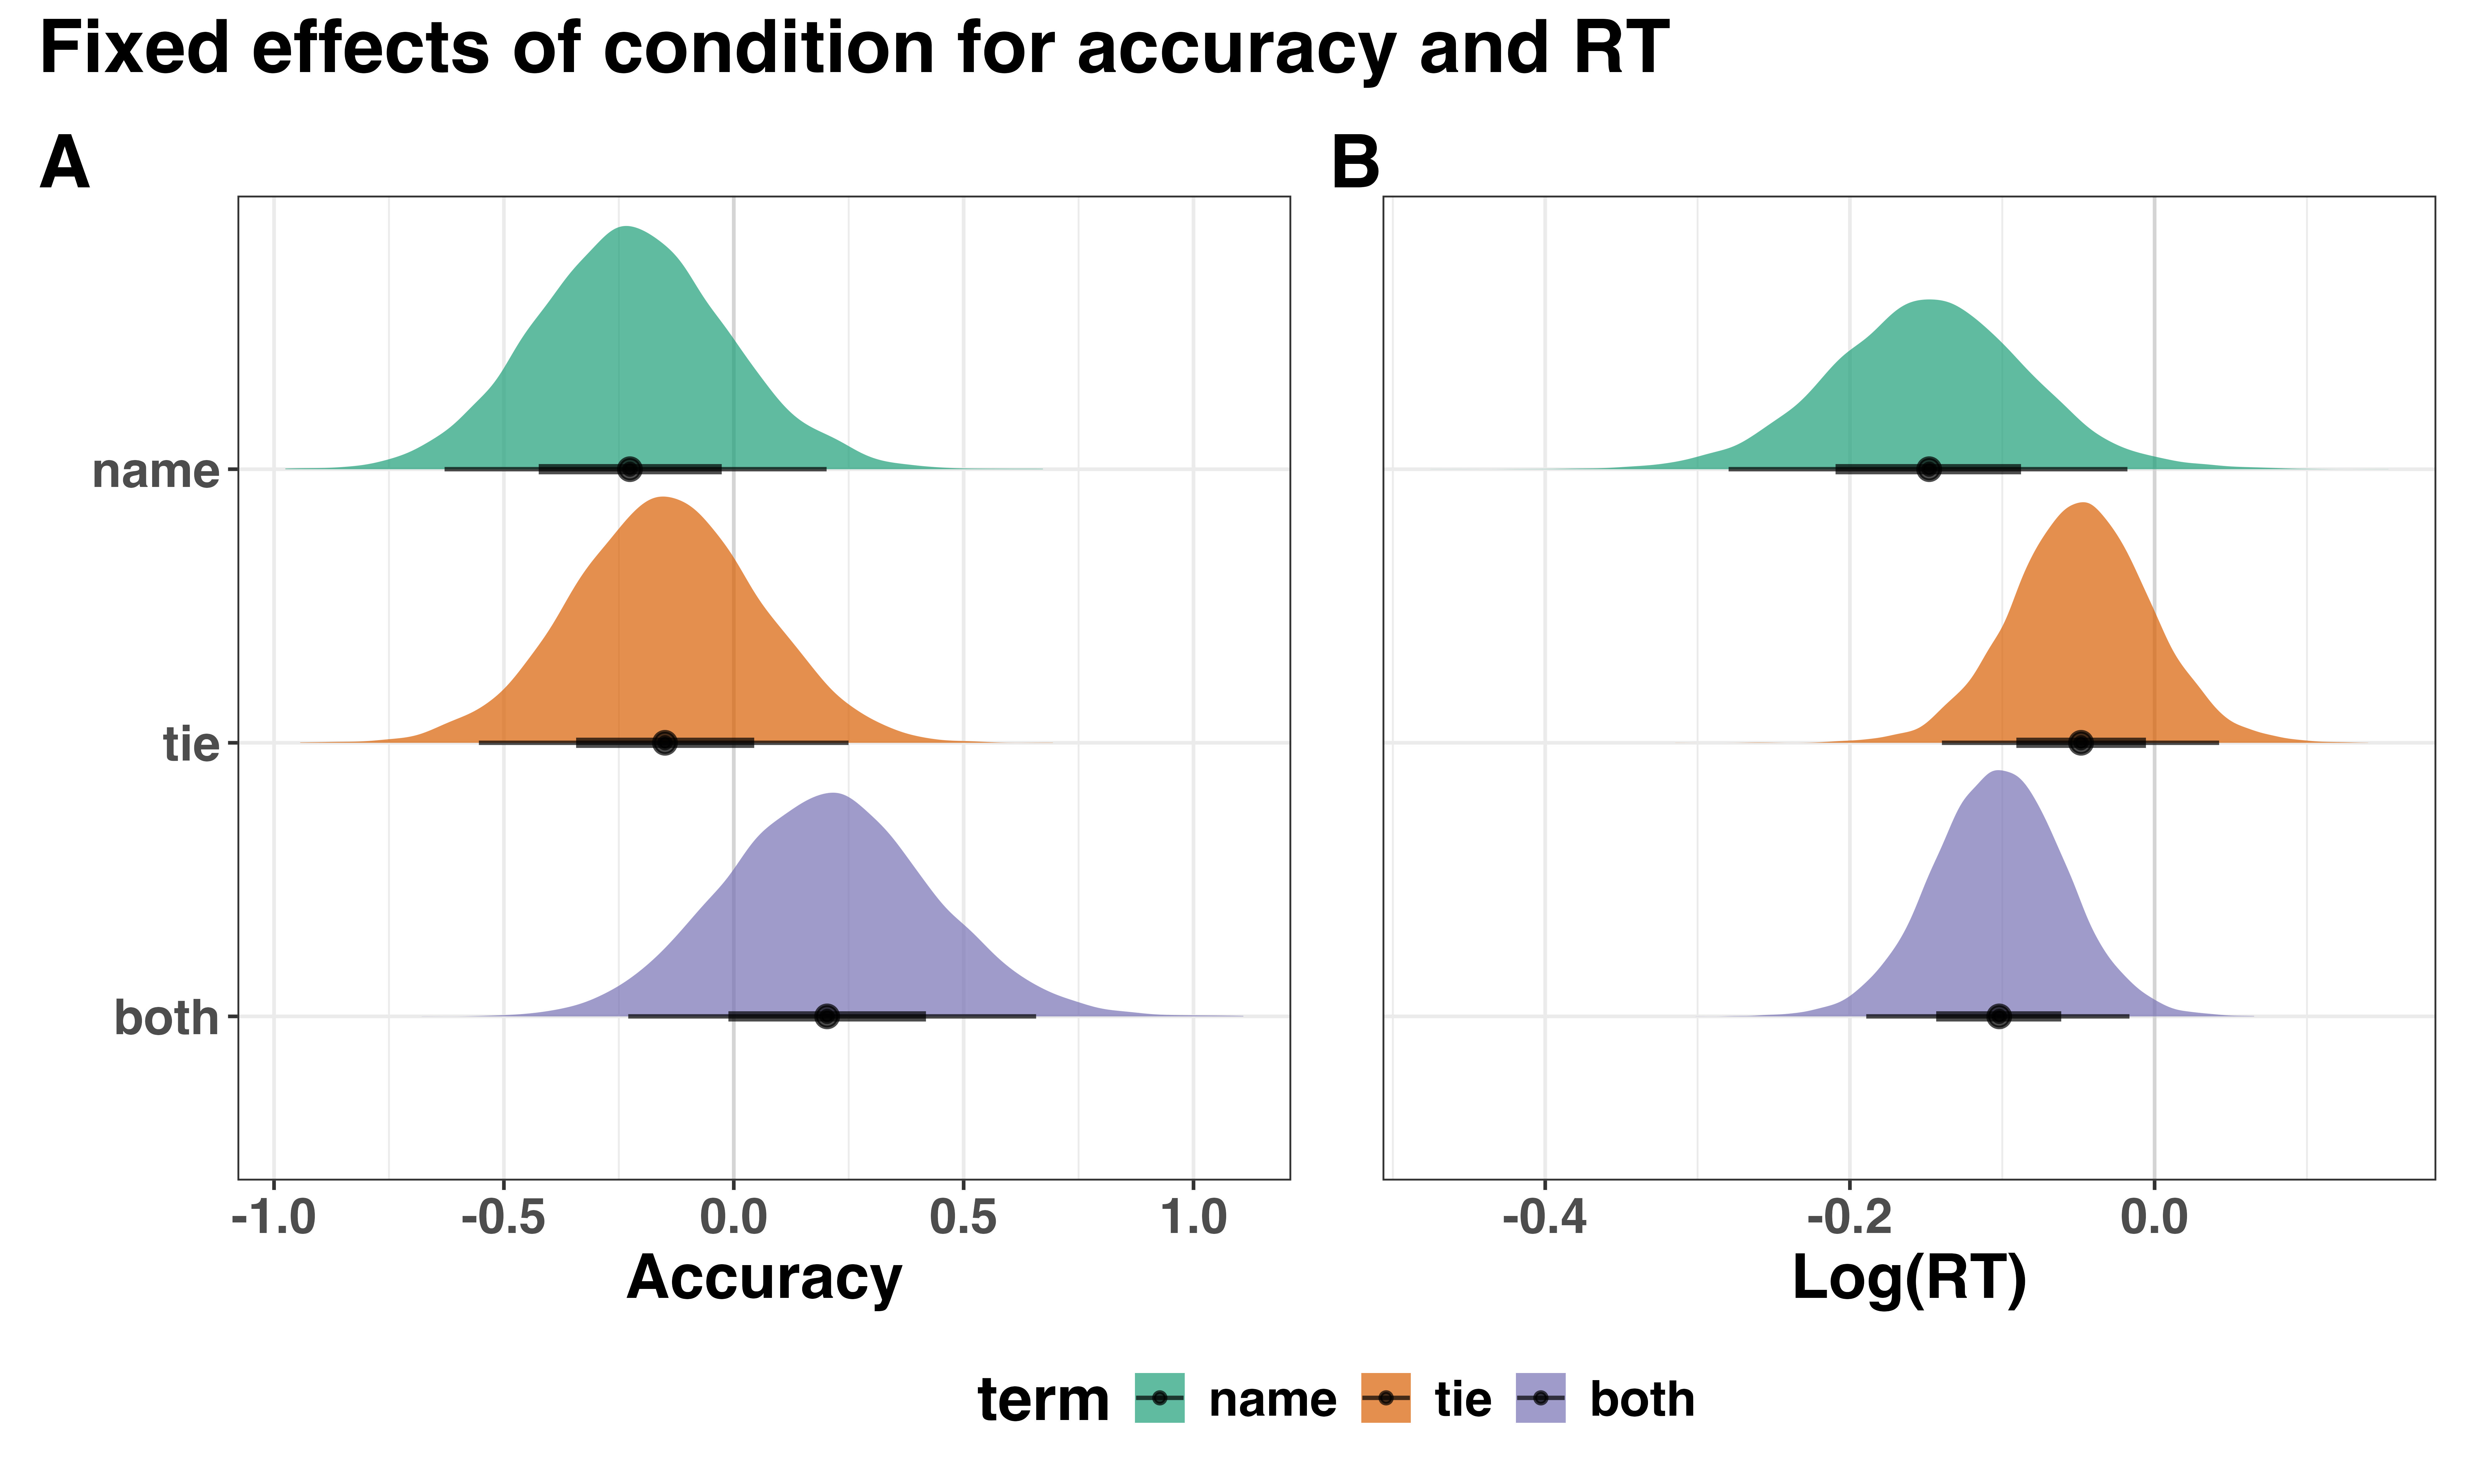
\includegraphics[height=0.67\textheight,]{../../figures/manifest/fixef} 

}

\caption{Fixed Effects for the Most Complex Model for (A) Accuracy and (B) Reaction Time. Points represent the median value of the posterior distribution for that estimate, the thicker line represents 66th percentile, while the thinner line is the 95th percentile of the distribution. The untrained condition was the reference group in these regression models.}\label{fig:fixef-plot}
\end{figure}

\subsubsection{Day 1, Session 1 Data}\label{day-1-session-1-data}

We also visually checked for any clear and obvious differences between training conditions that could have existed before any training had occurred (see Supplementary Figure 2).
In other words, we checked for random pre-training differences in RT and accuracy that might have existed in the Day 1, Session 1 data.



\begin{figure}[H]

{\centering 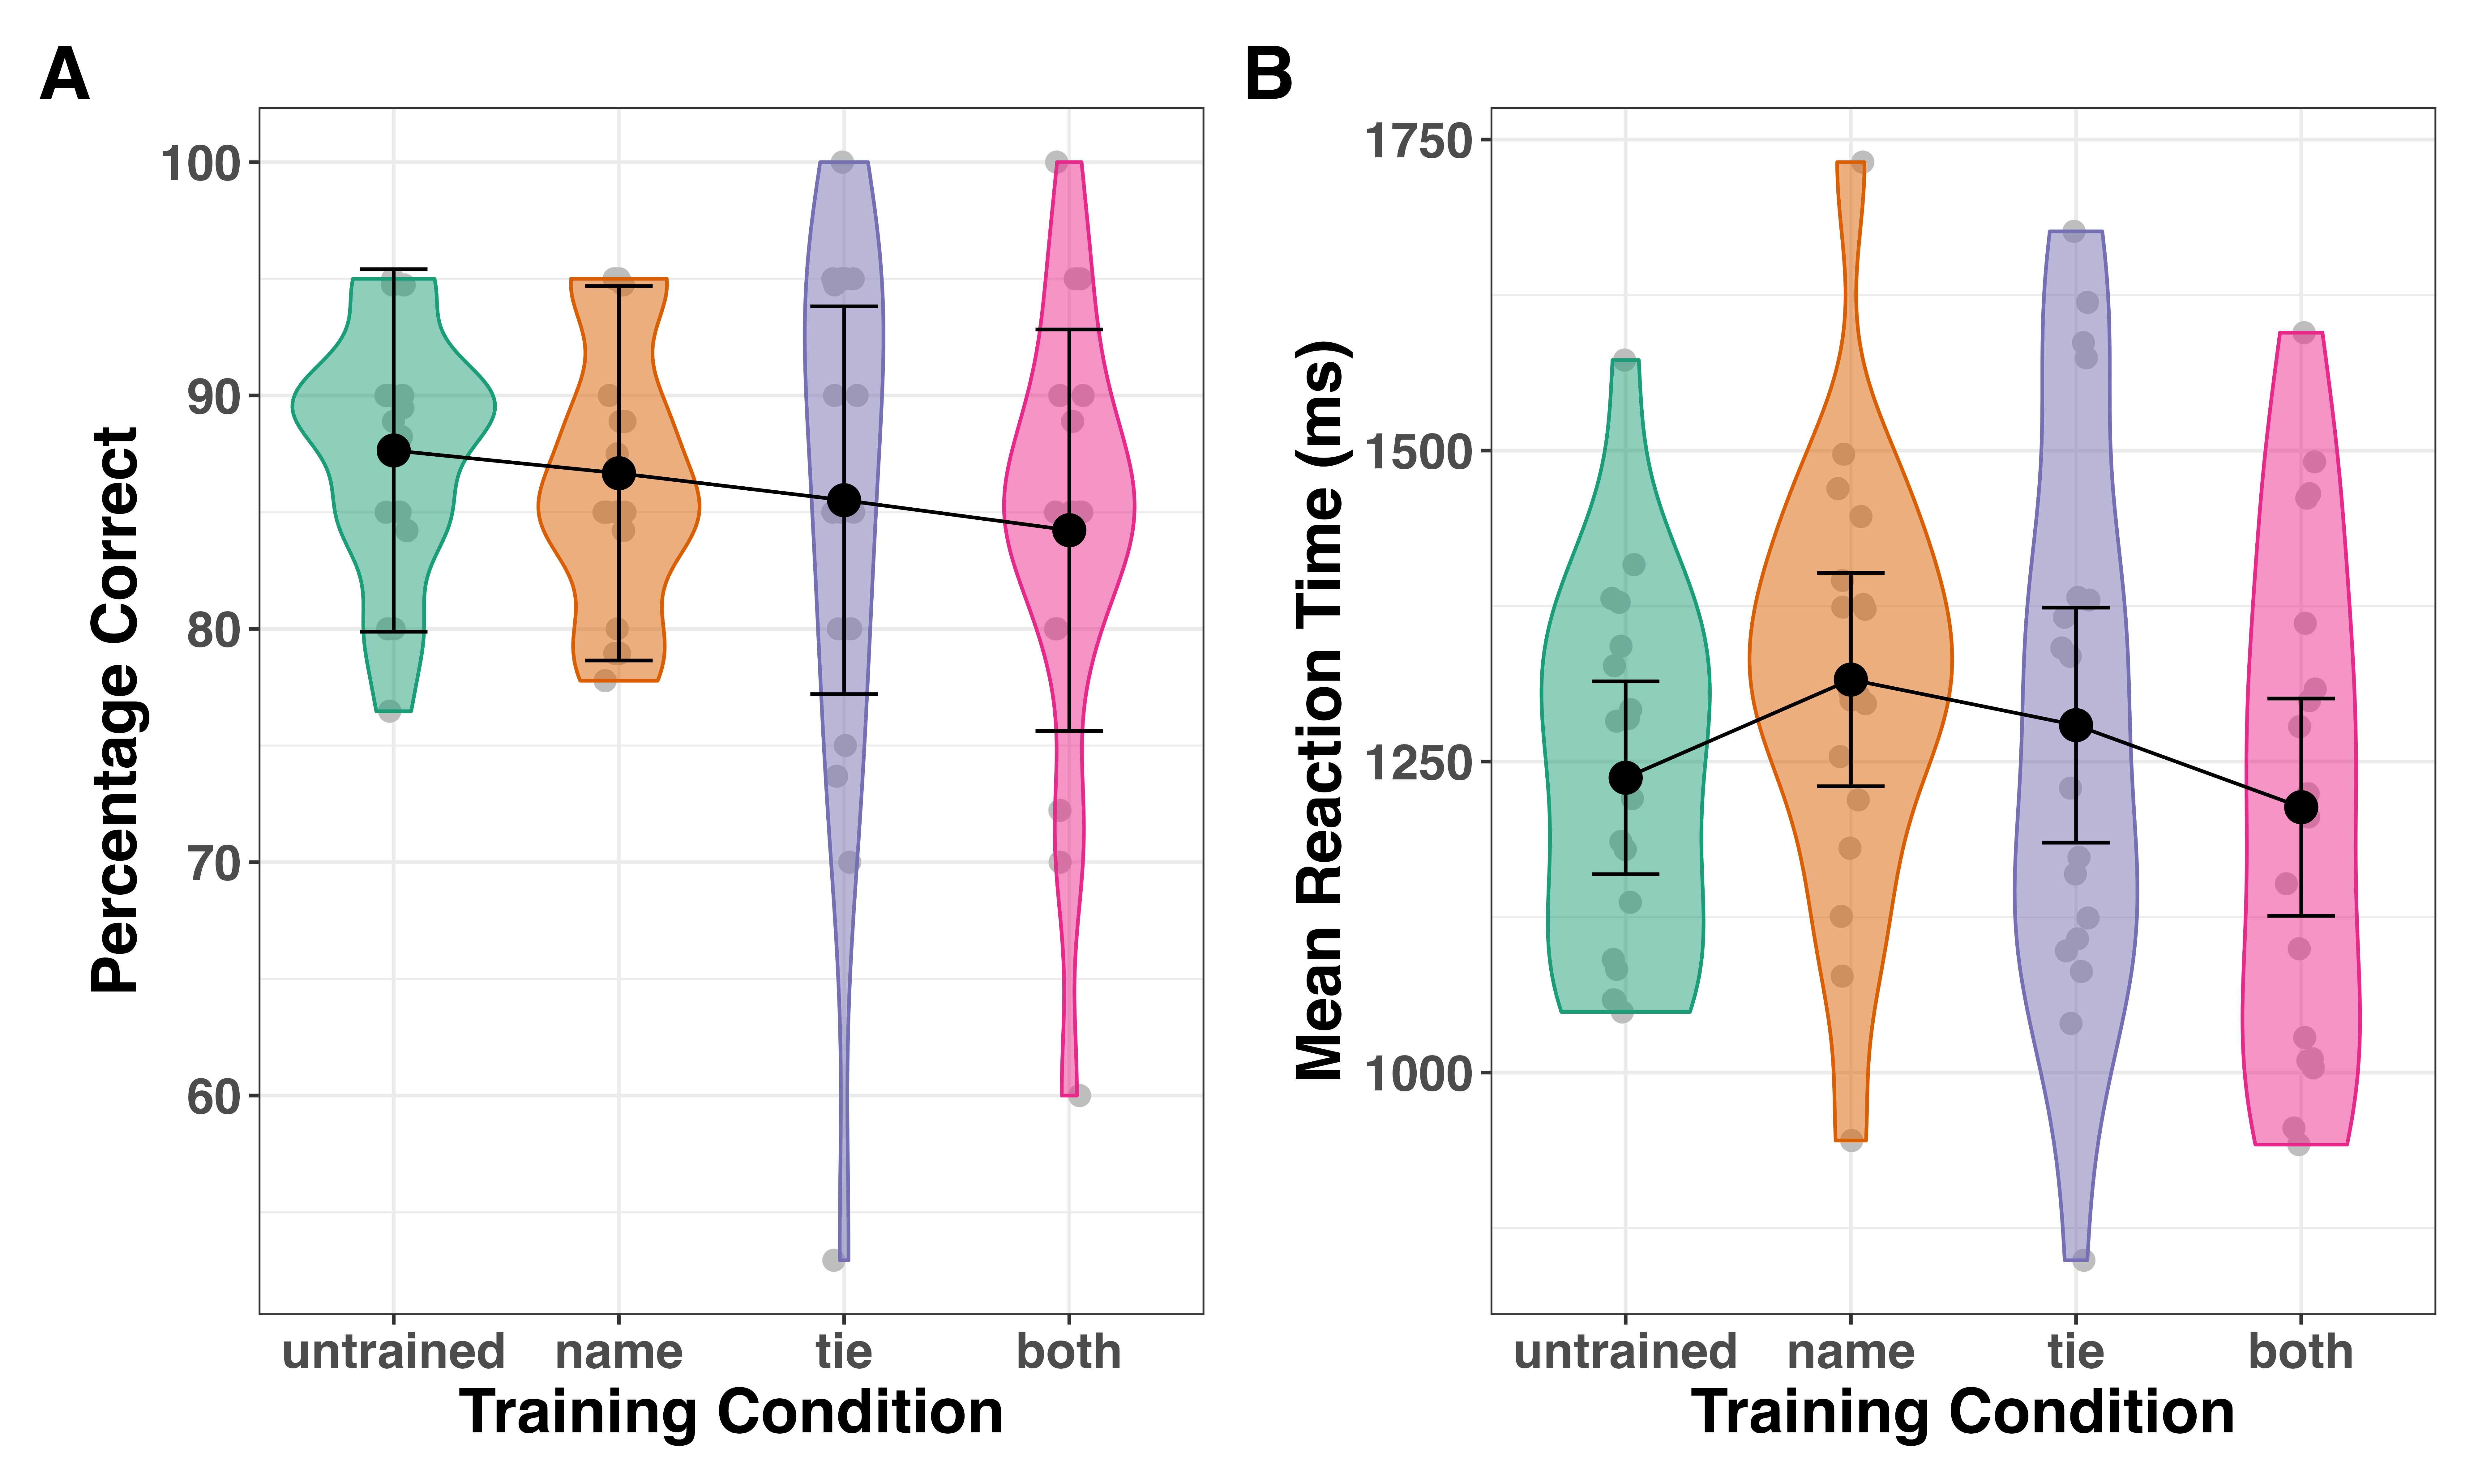
\includegraphics[height=0.67\textheight,]{../../figures/descriptive/day1_session1_violin_acc_rt} 

}

\caption{Accuracy and Reaction Time by Training Type for the Day 1 and Session 1 data (i.e., before any training had occurred). (A) Percent correct on the perceptual discrimination task by training type. (B) Mean reaction time (ms) on the perceptual discrimination task by training type. Black points denote group means, while error bars represent within subjects' standard errors of the mean. Grey points denote individual subject means.}\label{fig:day1-plot}
\end{figure}

At least in terms of accuracy and RT when analysed separately, there appears to be no clear and obvious pre-training differences between the conditions. Moreover, for RTs, any small numerical differences between conditions are in the opposite direction to the effect of training that we observed in RT, which is that trained conditions became faster than the untrained condition. Therefore, it seems unlikely that pre-existing, chance differences between conditions could account for our findings.

\subsection{LBA Analysis}\label{lba-analysis}

\subsubsection{Sampling}\label{sampling}

As much as possible, we used settings that were recommended for hierarchical sampling by the authors of the DMC software (Heathcote et al., 2019). Sampling was carried out in two steps. First, sampling was carried out separately for individual participants in order to get reasonable start points for hierarchical sampling. The results of this step were then used as starting points for sampling the full hierarchical sample. During the initial burn-in-period there was a probability of .05 that a crossover step was replaced with a migration step. After burn-in only crossover steps were used and sampling continued until the proportional scale reduction factor (\(\hat{R}\)) was less than 1.1 for all parameters, and also the multivariate version was less than 1.1 (Brooks \& Gelman, 1998). Hierarchical estimation assumed independent normal population distributions for each model parameter. Population-mean start points were calculated from the mean of the individual-subject posterior medians and population standard deviation from their standard deviations, with each chain getting a slightly different random perturbation of these values. Hierarchical sampling used probability .05 migration steps at both levels of the hierarchy during burn in and only crossover steps thereafter with thinning set at 10 (i.e., only every 10th sample was kept), with sampling continuing until \(\hat{R}\) for all parameters at all levels, and the multivariate \(\hat{R}\) values, were all less than 1.1. The final set of chains were also inspected visually to confirm convergence. For each model we used three times as many chains as model parameters.

\subsubsection{Priors}\label{priors}

Priors were chosen to have little influence on estimation. Priors were normal distributions that were truncated below zero for B, A and sv parameters, and truncated at 0.1s for the t0 parameter (assuming that responses made in less than 0.1s are implausible). The t0 parameter was truncated above by 1s. There were no other truncations, so the v prior was unbounded. The prior mean for B was 1 and for A 0.5. The v parameter for the true accumulator was given a prior mean of 1, while the mismatching accumulator was given a prior mean of 0. The sv parameter for the matching accumulator had a prior mean of 0.5. The t0 parameter had a prior mean of 0.2s. All priors had a standard deviation of 2. Mean parameters of population distributions were assumed to have priors of the same form as for individual estimation, and the standard deviations of hyper parameters were assumed to have exponential distributions with a scale parameter of one.





\begin{table}[tbp]

\begin{center}
\begin{threeparttable}

\caption{\label{tab:prior-lba-table}Priors used for the LBA analysis.}

\begin{tabular}{lllll}
\toprule
parameter & \multicolumn{1}{c}{mean} & \multicolumn{1}{c}{sd} & \multicolumn{1}{c}{lb} & \multicolumn{1}{c}{ub}\\
\midrule
A & 1 & 2 & 0 & -\\
B & 0.5 & 2 & 0 & -\\
t0 & 0.2 & 2 & 0.1 & 1\\
mean\_v\_true & 1 & 2 & - & -\\
mean\_v\_false & 0 & 2 & - & -\\
sd\_v\_true & 0.5 & 2 & - & -\\
sd\_v\_false & 1 & - & - & -\\
st0 & 0 & - & - & -\\
\bottomrule
\addlinespace
\end{tabular}

\begin{tablenotes}[para]
\normalsize{\textit{Note.} A = start point; B = threshold; mean\_v\_true = mean drift rate for correct responses; mean\_v\_false = mean drift rate for incorrect responses; sd\_v\_true = standard deviation of the mean drift rate for correct responses; SD = standard deviation; lb = lower bound; ub = upper bound. Two variables were given constant values to enable model fitting and these were set as follows: sd\_v\_false = 1, st0 = 0.}
\end{tablenotes}

\end{threeparttable}
\end{center}

\end{table}

\newpage

Plots of prior and posterior distributions revealed strong updating (i.e., posteriors dominated priors), making it clear that the prior assumptions had little influence on posterior estimates (see Supplementary Figure 3).



\begin{figure}[H]

{\centering 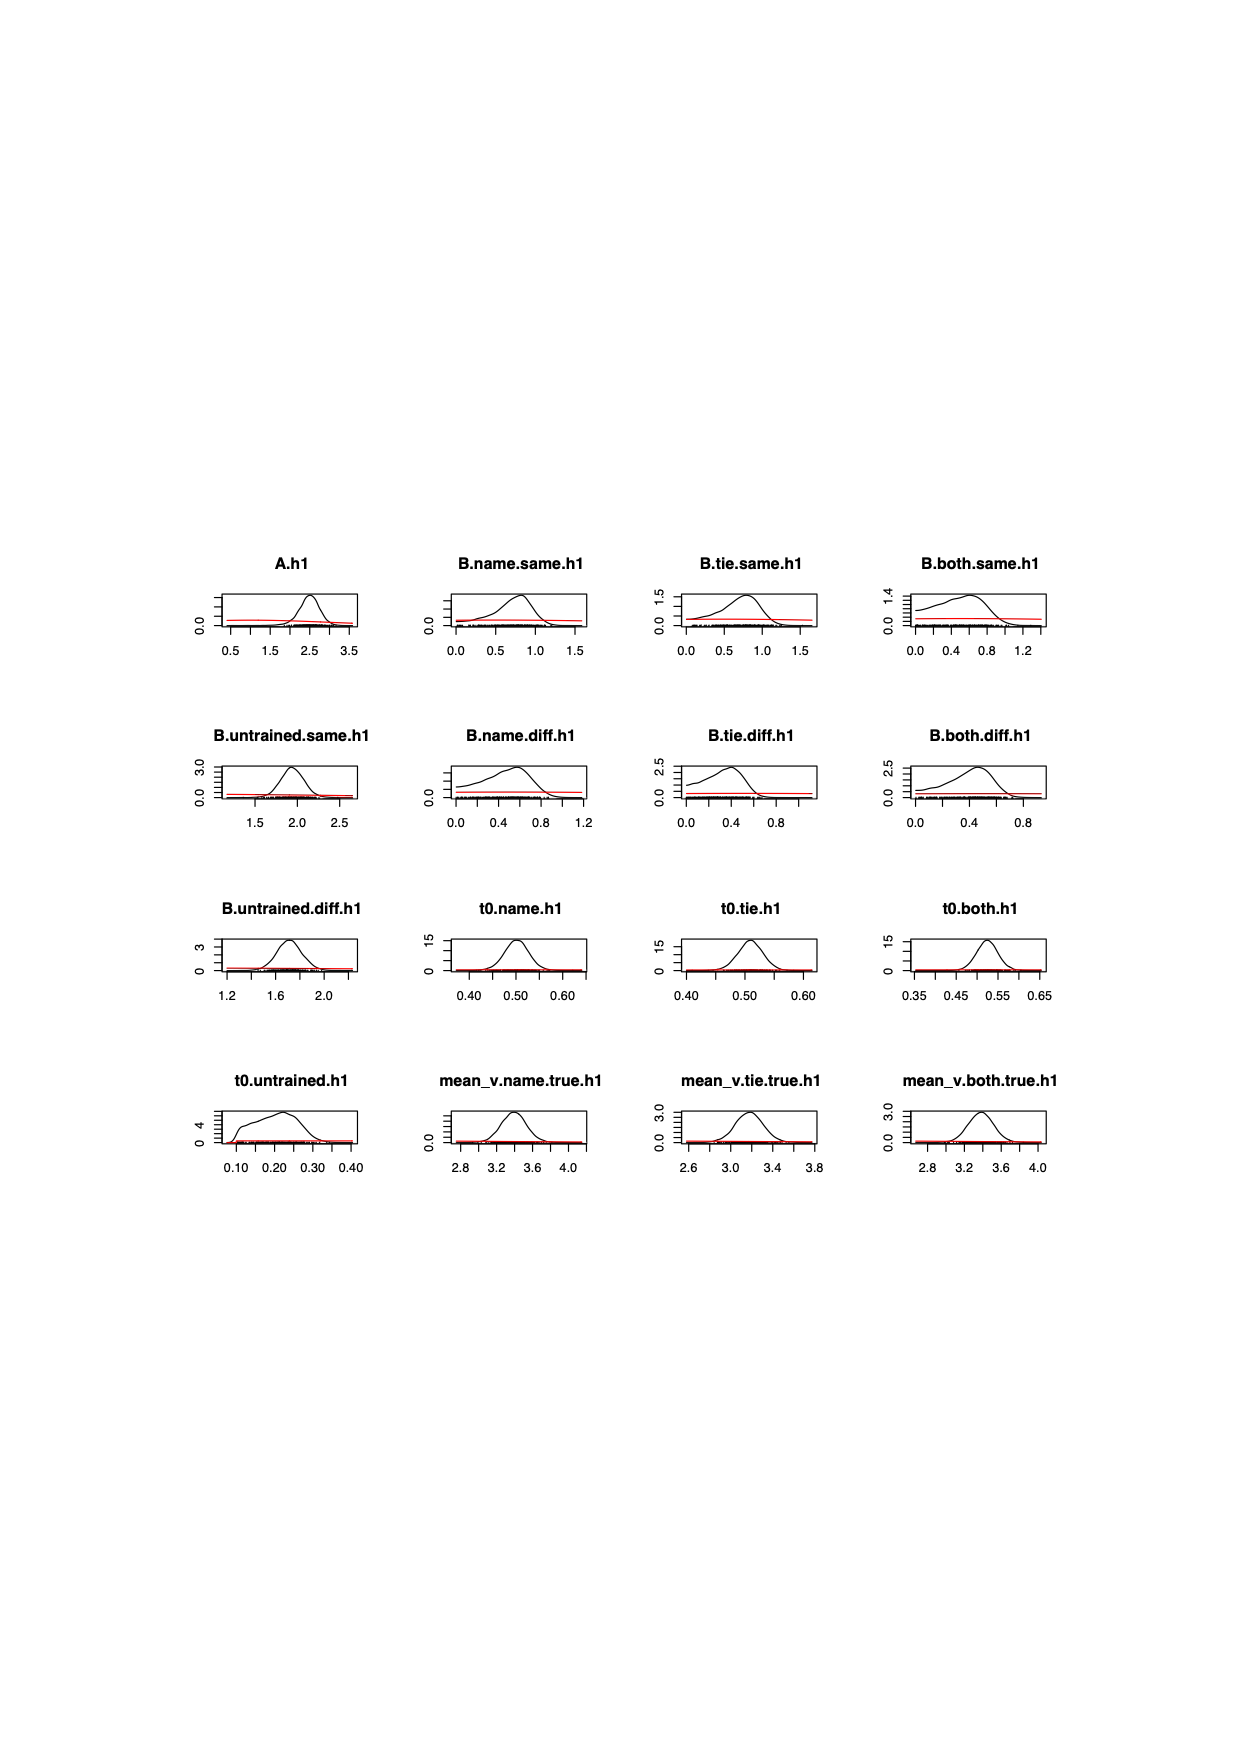
\includegraphics[height=0.67\textheight,]{../../figures/ea/pp} 

}

\caption{Prior and Posterior Graphs. Red lines represent priors, while black lines represent posteriors. Only a selection of all the parameters are shown here.}\label{fig:prior-post-plot}
\end{figure}

\subsubsection{Model fit}\label{model-fit}

Supplementary Figures 4 displays the fits of the LBA model to the data in terms of defective cumulative distribution functions (lines) and 10th, 30th, 50th, 70th and 90th percentiles (points from left to right) averaged over participants. Thick black lines and open points correspond to the data and the thin grey lines and solid black points correspond to the model predictions averaged over posterior samples. The grey points correspond to percentile predictions for 100 randomly selected sets of posterior parameter samples, so their spread gives an idea of the uncertainty in the model's predictions. As can be seen from the Supplementary Figure 4, the average fit of the selected LBA model was reasonable.



\begin{figure}[H]

{\centering 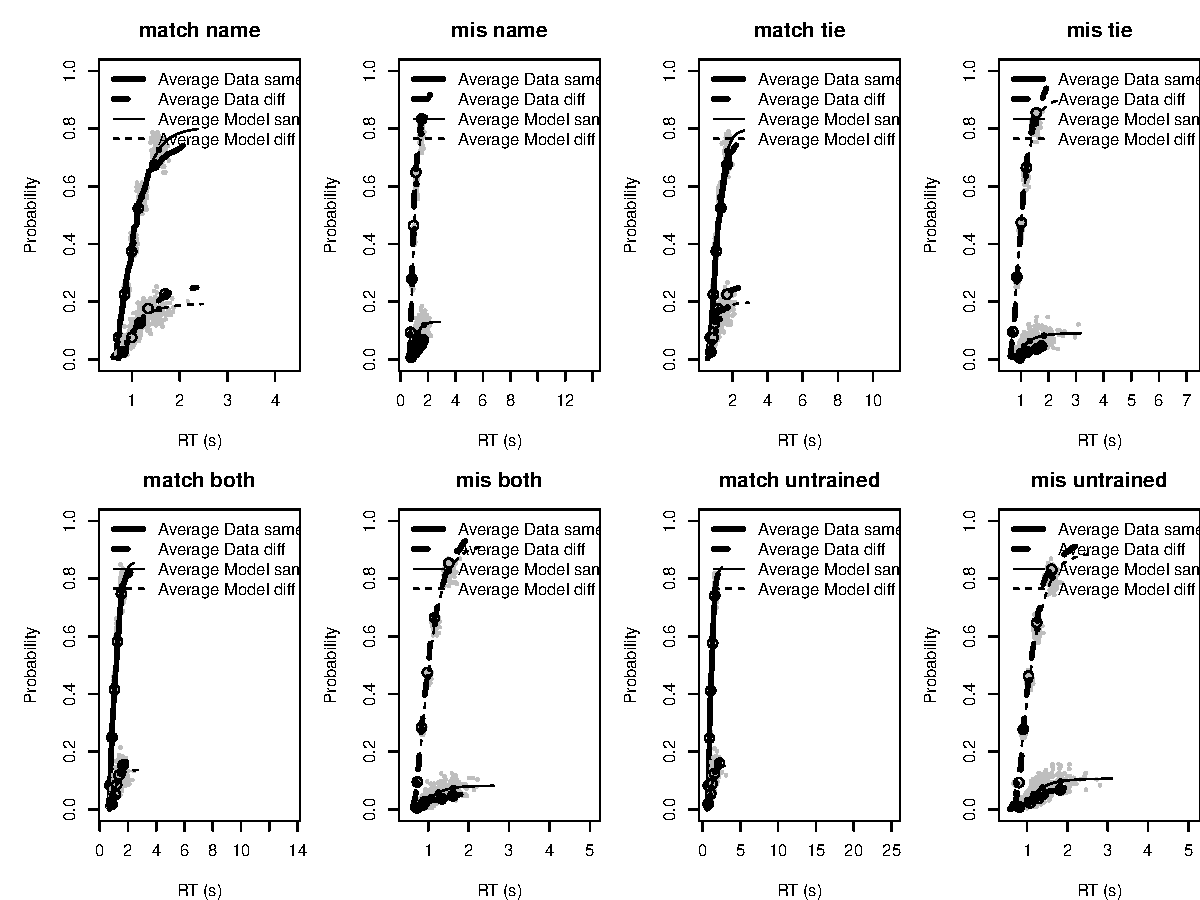
\includegraphics[height=0.67\textheight,]{../../figures/ea/KN_fit} 

}

\caption{Cumulative distribution functions for data (thick lines) and fits (line grey lines) of the LBA model. Each panel contains results for both same and different responses at each level of stimulus (match and mismatch) and training type (untrained, name, tie, both). Symbols mark the 10th, 30th, 50th, 70th and 90th percentile (solid for average fits, open for data). Grey points are 500 percentile estimates from fits for random draws from posterior samples; the grey line and black solid points are the average of these 500 fits.}\label{fig:model-fit-plot}
\end{figure}


\end{document}
